\section{Gamma-ray Attenuation}

\noindent In the Gosia manual, we have the following equations:

\begin{equation}
Q_k(E_\gamma) = {J_{k0}(E_\gamma) \over J_{00}(E_\gamma)}
\end{equation}

\begin{equation}
J_{k0}(E_\gamma) =
\int_0^{\alpha_{max}}
P_k(\cos\alpha)
\xi
K(\alpha)
\left(1 - exp(-\tau(E_\gamma) x(\alpha)\right)
\sin(\alpha)
d\alpha
\label{eq:jk0}
\end{equation}

where

\begin{equation}
K(\alpha) = 1 - exp^{-
\left(\sum_i \tau_i(E_\gamma) x_i(\alpha)\right)
}
\end{equation}

\noindent which describe the absorption of $\gamma$ rays in an
arbitrary shaped detector. The summation in the last equation extends
over all the absorbers and the inactive part of the detector (referred
to in the manual as the ``p-core''.\\

\noindent In the code, this is implemented for a coaxial detector.
Note, however, that gosia assumes a true coaxial geometry for the Ge
detector, which is not realistic. Real detectors have a closed front
end, to avoid having passivation at the point where the electrode
emerges from the crystal. Such passivation leads to a dead layer
around that point. A dead layer at the back of the crystal merely
reduces the efficiency, but at the front, it leads to a reduction of
peak-to-total.\\

\noindent In order to consider the absorption of $\gamma$ rays in the
detector, we divide it up into four regions as shown in figure
\ref{fig:atten}. A $\gamma$ ray in region 0 passes only through the
core and is not detected. A $\gamma$ ray in region 1 passes partly
through the core, where it might be absorbed, but then passes through
part of the crystal. So we need to consider the absorption by the
inactive core and then the detection probability in the rest. Region 2
is the simplest, as it passes only through active parts of the
detector until it reaches the back face. Region 3 also only passes
through active parts, but it reaches the side of the detector.\\

\begin{figure}[ht!]
\includegraphics[width=0.8\textwidth]{geometry_for_attenuation.ps}
\caption{Geometry for attenuation}
\label{fig:atten}
\end{figure}

\noindent The code is in the function {\em GCF}. Here we define four
angles corresponding to the four blue lines on figure \ref{fig:atten}.
Together with zero degrees, these bound the four regions. These angles
are stored in the array $b$.

\begin{center}
\begin{tabular}{|llll|}
\hline
Variable & Symbol & Value & Meaning\\
\hline
b(1) & $\alpha_1$ & $\arctan({a \over d + l})$ & Boundary between regions 0 and 1\\
b(2) & $\alpha_2$ & $\arctan({a \over d})$ & Boundary between regions 1 and 2\\
b(3) & $\alpha_3$ & $\arctan({r \over d + l})$ & Boundary between regions 2 and 3\\
b(4) & $\alpha_4$ & $\arctan({r \over d})$ & Boundary between regions 3 and 4\\
\hline
\end{tabular}
\end{center}

\noindent We expand the attenuation factor in terms of Legendre
polynomials going up to 8$^\textrm{th}$ order. Note that the index $k$
is the order plus one. i.e. $k$ in the code is one more than $k$ in
the formulae! This is because it is also used to index Fortran arrays.
These polynomials are hardcoded in {\em GCF}.\\

\noindent So we loop over the order of the Legendre polynomial and
then over the regions, leaving out region 0, because nothing is
detected there. Then we subdivide each region into 100 slices and for
each calculate the angle $\alpha$ which we store as {\em xm}.\\

\noindent We need to calculate the absorption factor for the length of
crystal seen by the $\gamma$ ray, assuming an attenuation coefficient
$\tau$. This is different for each region.\\

\noindent We calculate the integrand of \ref{eq:jk0} for the 100
slices and then use Simpson's rule to integrate. i.e.

\begin{equation}
\int_a^b f(x) dx \sim {h \over 3}
\left[
f(x_0)
+ 2 \displaystyle\sum_{j = 1}^{n/2 - 1} f(x_{2j})
+ 4 \displaystyle\sum_{j = 1}^{n/2} f(x_{2j-1})
+ f(x_n)
\right]
\end{equation}

\noindent After we have evaluated $J_{k0}$ for k = 0{\ldots}8, we can
evaluate $Q_k$.

\subsection{Region 1}

\noindent In this region, the $\gamma$ ray hits the front face of the
crystal at a radius from the centre which is less than the core
radius, given by $d\tan\alpha$. It then passes through the core,
emerges from the core and continues until the back face. The path length
within the core is given by $a - d\tan\alpha\over\sin\alpha$ = 
${a\over\sin\alpha} - {d\over\cos\alpha}$.\\

\noindent The distance from the point where the $\gamma$ ray hits the
front face, to where it reaches the back face is given by $l \over
\cos\alpha$. So the distance in the active part is given by
${l \over \cos\alpha} - \left({a\over\sin\alpha} -
{d\over\cos\alpha}\right)$ =
${d + l \over \cos\alpha} - {a\over\sin\alpha}$ = 
${(d + l) \tan\alpha - a \over \sin\alpha}$. So the absorption factor
is given by $e^{-{\left((d + l) \tan\alpha - a \over
\sin\alpha\right)\tau}}$.

\subsection{Region 2}

\noindent In this region, the path length from the point where the
$\gamma$ ray hits the front face to the point where it reaches the
back face, is $l \over \cos\alpha$. So the absoption factor is given
by $e^{-{l \tau \over \cos\alpha}}$.

\subsection{Region 3}

\noindent In this region, the $\gamma$ ray hits the front face at a
radius $d\tan\alpha$ from the centre, or $r - d\tan\alpha$ from the
edge. So the distance travelled in the crystal from this point to the
side of the detector is ${r - d\tan\alpha \over\sin\alpha}$. So the
absorption factor is $e^{-{r - d\tan\alpha \over\sin\alpha}\tau}$.
